This thesis investigates stellar streams originating from globular clusters in the Milky Way. Stellar streams are long, thin structures composed of stars that have escaped their parent clusters, forming coherent trails that can span large regions of the sky. Globular clusters—dense, gravitationally bound systems containing hundreds of thousands to millions of stars—are particularly prolific sources of such streams. In Chapter 4, I present the first study to simulate streams from the entire Galactic globular cluster system, using realistic initial conditions (mass, size, position, and velocity) and an axisymmetric, time-independent model of the Milky Way's gravitational potential. Chapter 5 builds on this work, exploring how the collective gravitational influence of all globular clusters can perturb stellar streams, producing underdensities known as ``gaps''. These features are of central interest in the field, as they may encode information about the dark matter distribution in the Galaxy.

The structure of the thesis is as follows. The remainder of this introductory chapter provides background on stellar streams, globular clusters, and their astrophysical context, as well as an overview of the current state of the field. Chapter~2 outlines the physical framework used to model stream formation and interpret their morphology. Chapter~3 describes the numerical methods employed in the simulations, including convergence tests and estimates of computational cost. Chapters~4 and~5 present two published studies, with the final chapter discussing these results in the broader context of the literature and highlighting future directions.

\section{General context}

    Before I explain why it is scientifically interesting to study such objects, I must first lay out the scene. This thesis fits neatly in the field of galactic astronomy, which, in essence, is the study of the state of our very own galaxy and how it came to be within the larger universe.

    A natural starting point of this narrative is the beginning of the universe. Essentially, just a few minutes after the Big Bang, conditions were favorable enough to allow protons and electrons to exist. For a few minutes, these particles collided with one another to fuse into heavier elements. This phase of the universe is known as Big Bang Nucleosysntehsis \citep{2007ARNPS..57..463S}. They mostly hydrogen, deuterium $^2$H, $^4$He, and some trace amounts of $^3$He and $^7$Li. By mass, the composition of the universe was 75~\% Hydrogen and 25~\% Helium \citet{1966ApJ...146..542P,2016RvMP...88a5004C}. 

    Dark matter constitutes approximately five times more mass than ordinary (baryonic) matter in the universe \citep{2020A&A...641A...6P}. In the early universe, dark matter was distributed nearly uniformly, but gravitational instabilities caused it to coalesce and form the cosmic web. The nodes of the web are very massive and contain deep gravitational potential wells that attracted surrounding ordinary material. This infalling gas subsequently formed stars. The resulting assemblage of stars, gas, and dark matter constitutes a galaxy \citep{2008LNP...740.....P,2010gfe..book.....M}. In certain situations, the star 

    The universe contains not just a single galaxy, but a vast population of them. According to the $\Lambda$CDM paradigm, cosmic structure formed hierarchically, with small protogalaxies merging over time to build larger systems \citep{2015ARA&A..53...51S}. 

    As galaxies evolve, their stars fuse hydrogen and helium into heavier elements, enriching the interstellar medium with each generation. Massive stars live short lives and often end in supernovae, ejecting enriched material back into their surroundings. This gas can then collapse to form new stars. When galaxies interact or merge, their gas mixes, further driving star formation and chemical enrichment \citep{2019A&ARv..27....3M}.
    
    When stars are made, in many circumstances, they may not just form single stars but clusters of stars. These star clusters come to be when many stars form at once and are also bound to each other gravitationally. One of the most essential objects in this thesis is globular clusters, which are clusters containing hundreds of thousands to millions of stars. 

    These star clusters, or any extended object that orbits around a larger host, experience tidal forces. There are many examples of this in nature. The most familiar example is how the lunar tides control the water. But for this work, we are interested in more extreme tidal forces, those that are strong enough to disintegrate a body. For example, some hypotheses say that Saturn's rings come from a body that was ripped apart by Saturn's tidal field and then became a collection of rocks and dust \citep{2009Icar..199..413C}. Also, tidal forces played a pivotal role in the Earth-Moon formation scenario; an excellent visualization of the  code SWIFT \url{https://swift.strw.leidenuniv.nl/about.html} \citep{2024MNRAS.530.2378S}, as the proto-moon came to close to the earth, the tidal forces disintegrated it, the earth absorbed a portion and a portion distanced itself from the world to create the moon.

    Those are examples in which the tidal forces rip apart solid bodies. However, star clusters are not solid objects but are instead composed of many stars that are bound together gravitationally. The tidal forces disintegrate star clusters in a much more gentle way. The tidal forces inject enough energy to gently and slowly pull the cluster apart. A result is that the stars that escape from the cluster have more or less the same orbit as the cluster's center of mass \citep{1972ApJ...178..623T,1995AJ....109.2553G}. As the system moves along, the stars coherently spread out along one orbital trajectory and create stellar streams. See Fig.~\ref{fig:S5MilkywayStreams}. 

    \begin{figure}
        \centering
        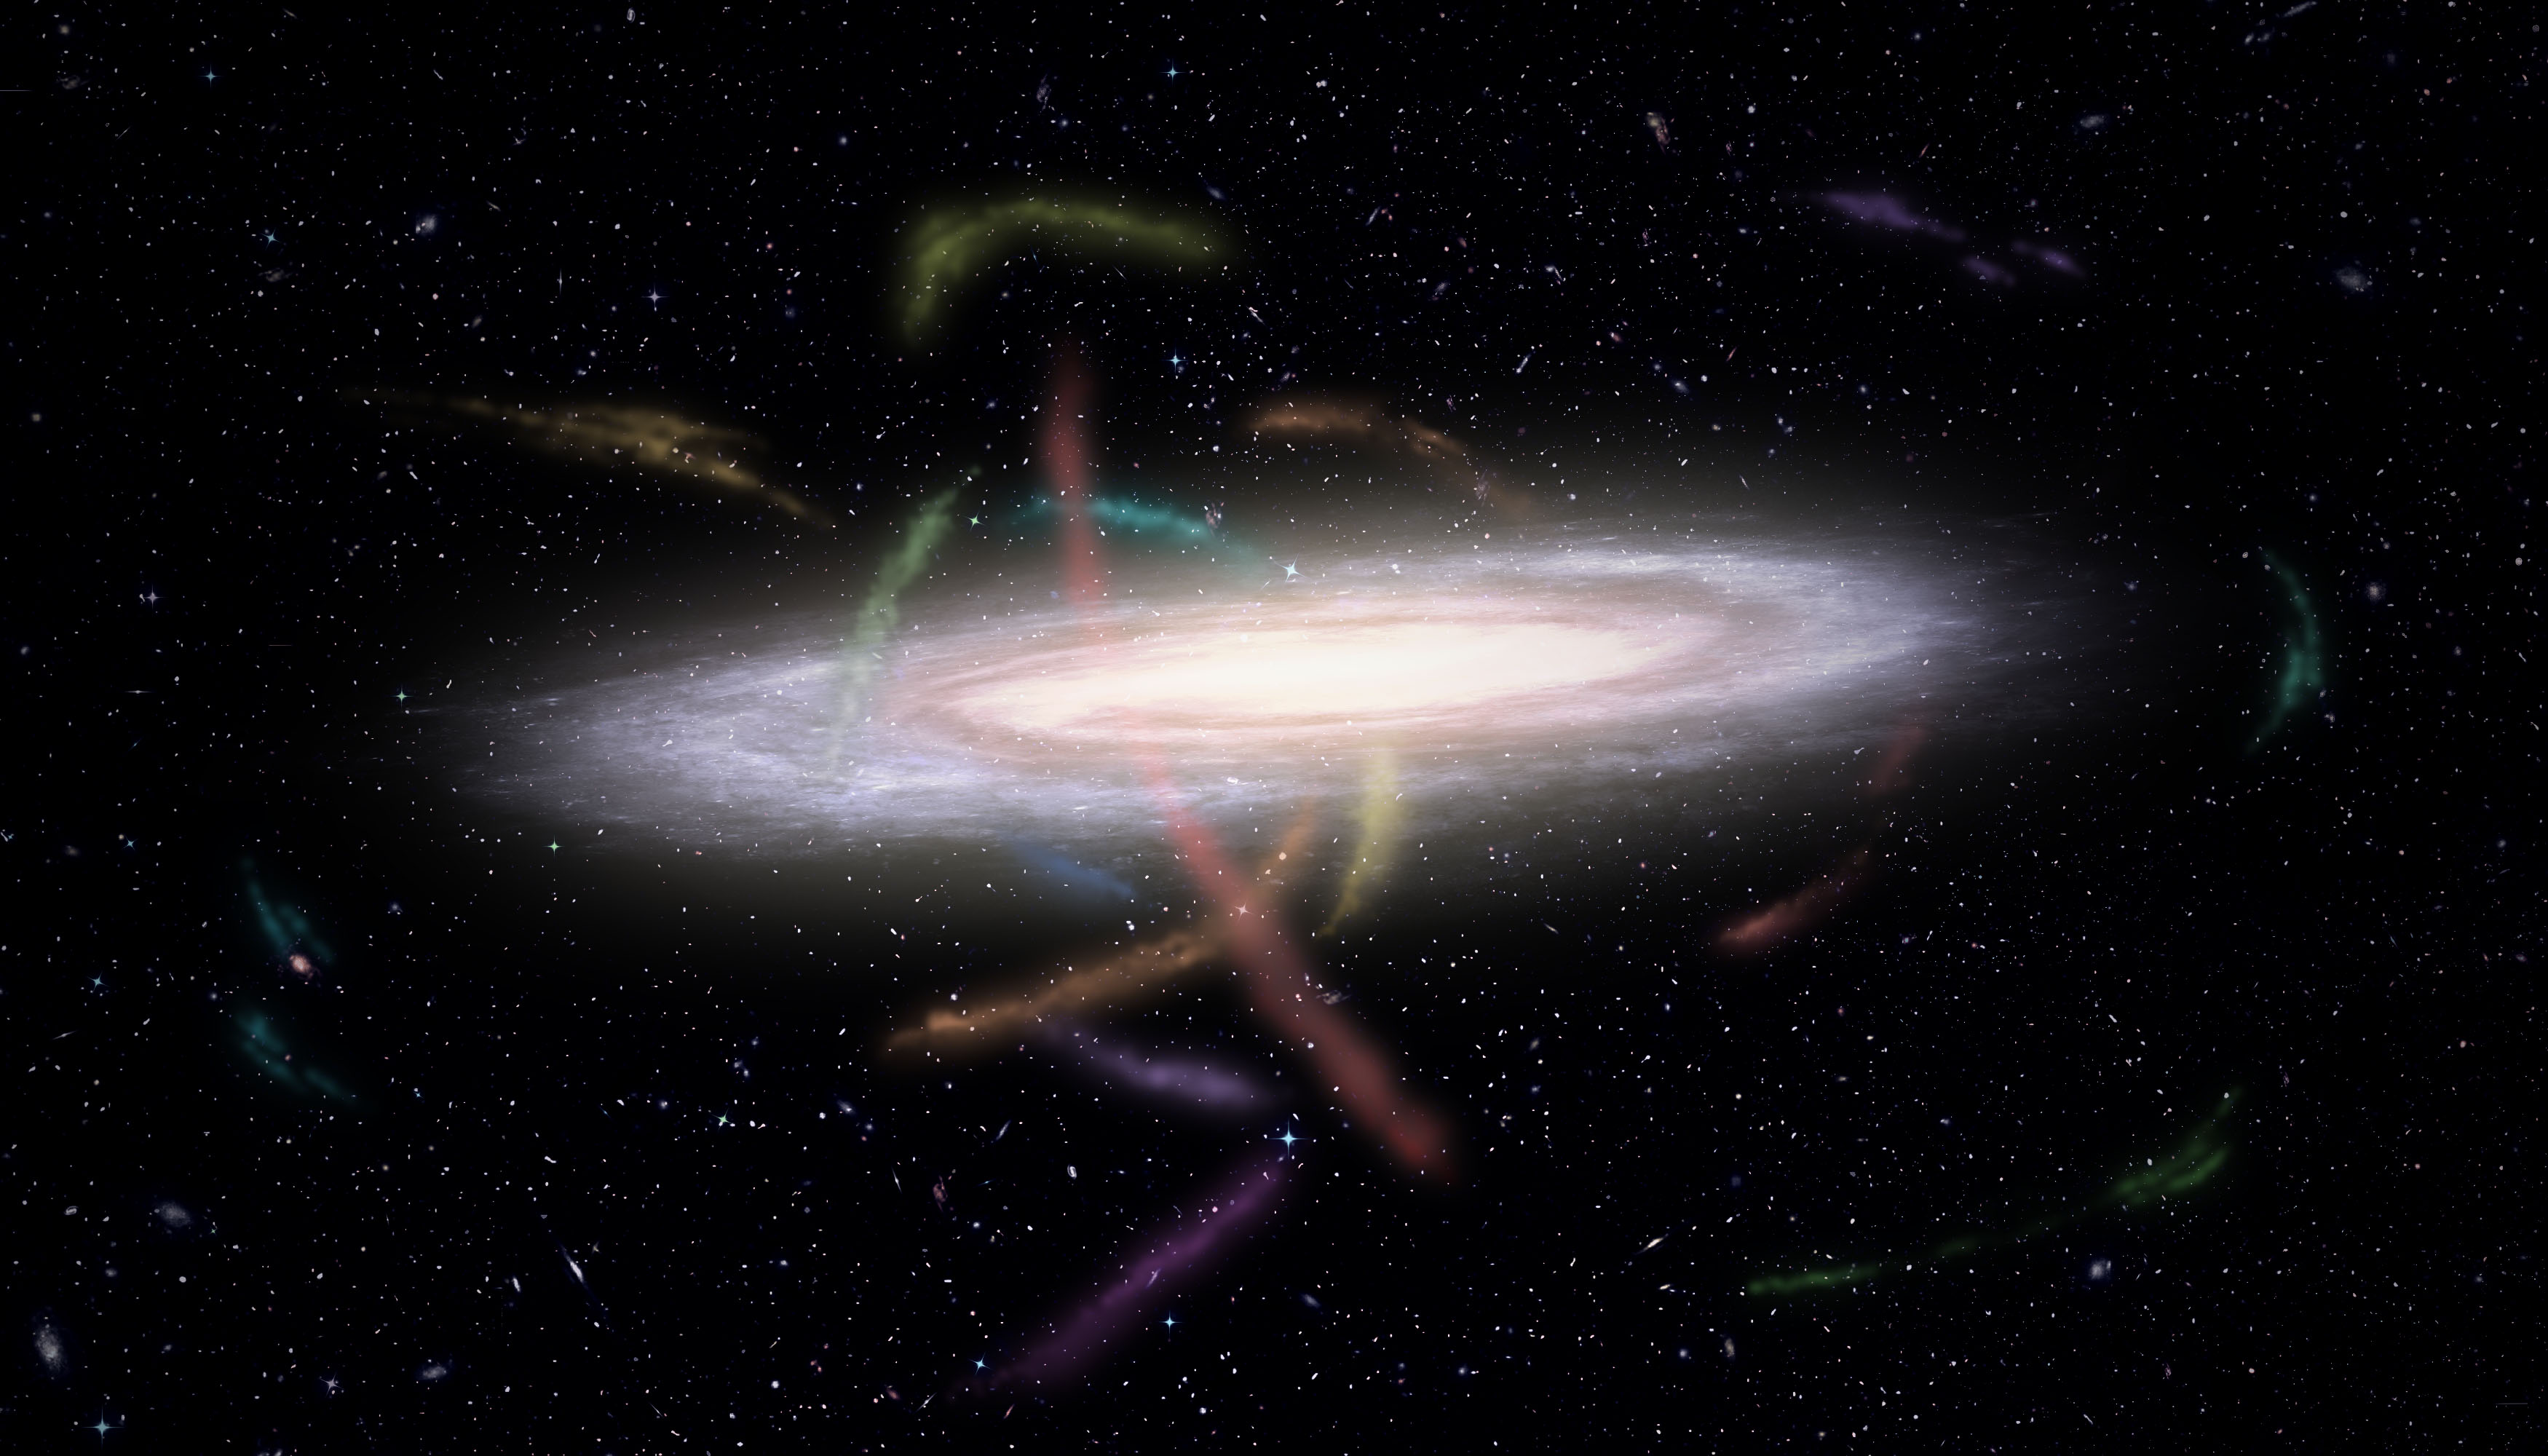
\includegraphics[width=\linewidth]{images/S5MilkywayStreams.jpg}
        \caption{An artist's rendition of a galaxy surrounded by stellar streams. Credit: James Josephides and S$^5$ Collaboration \citep{2019MNRAS.490.3508L}.}
        \label{fig:S5MilkywayStreams}
    \end{figure}

    Globular clusters are among the oldest stellar systems in the universe and thus serve as invaluable fossil records of early star formation \citep{1992ApJ...400..265M}. With the universe's age estimated at approximately 13.8 billion years, these clusters provide insights into conditions prevalent during the universe's formative epochs. Observationally, globular clusters display properties characteristic of single stellar populations \citep{1970ApJ...162..841S}, meaning their constituent stars formed nearly simultaneously from chemically homogeneous material, though with a range of stellar masses. Stellar evolution within these clusters is predominantly driven by mass, with more massive stars evolving more rapidly. This progression manifests clearly in color-magnitude diagrams, allowing age determinations of stellar populations. For Milky Way globular clusters, typical age estimates fall between 8 and 12 billion years \citep{2013ApJ...775..134V}.

    Globular clusters and their associated stellar streams offer many powerful avenues for astrophysical investigation. First, because direct observations provide only a snapshot of the universe at present, astrophysical phenomena evolving over timescales vastly exceeding human lifespans remain challenging to study. For instance, the Sun takes roughly 220 million years to complete a single orbit around the Galaxy. Stellar streams, by encoding orbital trajectories of their progenitor clusters, provide a unique window into millions of years of dynamical history. By characterizing their shapes and extents, we gain precise constraints on the Galactic gravitational potential.

    Second, as relics of the early universe, globular clusters encode critical information about their formation environments. For this reason, the field of study is often referred to as ``galactic archaeology'', as globular clusters serve to astronomers much like fossils do to archaeologists. Their properties reveal details about the interstellar medium at the time of their formation, as well as the Galaxy's assembly history \citep{2021ApJ...909L..26B,2023A&A...673A..86P}. Some Milky Way globular clusters formed in situ, while others were accreted from satellite galaxies or formed during merger events.

    Third, globular clusters serve as natural laboratories for studying the interplay of diverse physical processes. Their evolution involves stellar structure and evolution, gravitational dynamics, and relativistic effects in dense environments. For instance, close stellar encounters and binary interactions—such as mass transfer or mergers—are common in such environments and significantly shape cluster evolution \citep{2004MNRAS.349..129D,2016MNRAS.458.1450W,2024MNRAS.528.5119A}. 

    Globular clusters are also prime candidates for hosting intermediate-mass black holes (IMBHs) \citep{2013MNRAS.432.2779B,2015MNRAS.454.3150G}. The origin of IMBHs remains uncertain, as their masses are too large to be explained by isolated stellar evolution, yet too small to fall into the supermassive category \citep{2020ARA&A..58..257G}.

    Furthermore, while globular clusters were once thought to consist of single stellar populations, detailed observations of chemical abundances have revealed the presence of multiple populations, with distinct patterns in light elements (i.e., carbon, oxygen, nitrogen). This phenomenon reflects a complex history of star formation, feedback, and internal dynamical evolution \citep{2008MNRAS.391..825D,2012A&ARv..20...50G,2018ARA&A..56...83B}. 

    Lastly, globular clusters are everywhere in the universe \citep{2006ARA&A..44..193B,2019ARA&A..57..227K}. They are observed far in the past (the high redshift universe), and have though to have been more numerous but yet many of them persist until today. Not only this but they properties of a globular cluster system is tightly related to it's host galaxy. Additionally, it has been demonstrated that extra galactic stellar streams, even with just projected information (latitude and longitude), some parameters of the gravitational field can be recovered \citep{2011MNRAS.417..198V, 2023ApJ...954..195N}. 

    Thus, the stellar streams and globular clusters contain much information that can inform us various aspects of fundamental phyiscs our own galaxies, neighboring galaxies, and the past, and they can give us information about the current dynamical state of the galaxy. 


% \section{The Gaia Era}
%     \begin{itemize}
%         \item This section will be much more techical 
%         \item Present some gaia data products 
%         \item present the globular cluster catalogue
%         \item present eugenes work of the DR3 view of globular clusters 
%         \item present Rodrigo's work on detecting the stellar streams 
%     \end{itemize}


%   Stellar streams are several-kiloparsecs-long structures formed by the tidal disruption of globular clusters or dwarf galaxies orbiting a host galaxy. These tidal forces arise due to differential gravitational pulls across extended objects, causing stars farther from the galactic center to lag behind, while those closer to the center speed up. This stretching creates two tidal tails that trace the cluster's orbit unless in the closest vicinity to the object \citep{2007ApJ...659.1212M}. 
  
%   Numerical predictions of this phenomenon have existed since the 1970s \citep[see, e.g.,][]{1975AJ.....80..290K}. These predictions occurred well before the first detections of Galactic globular cluster tidal tails \citep{1995AJ....109.2553G}. Interestingly, \citet{1995AJ....109.2553G}'s detections were made nearly contemporaneously with the discovery of the Sagittarius stellar stream by \citet{1994Natur.370..194I}, which is the closest example of a stream emerging from a dwarf satellite currently interacting with the Milky Way. 
  
%   Subsequent studies\footnote{For more subsequent observation detections of tidal debris, i.e., globular cluster stars beyond the tidal radius see the works of: \citet{1997A&A...320..776L, 2000A&A...356..127T, 2000A&A...359..907L, 2001AAS...19910906S, 2003AJ....126..815L,2011ApJ...726...47S,2018MNRAS.476.4814S,2020MNRAS.495.2222S}.} extended Grillmair's findings to other globular cluster streams but were often limited to the detections of stars still close to the cluster tidal radius, until the discovery made by \citet{2001ApJ...548L.165O,2002AAS...200.1001O, 2003AJ....126.2385O} of long and thin tails outside the Palomar~5 globular cluster. With a mass of $1.34\pm 0.24 \times 10^4 M_{\odot}$ \citep{2019MNRAS.482.5138B}, Palomar~5 is one of the least massive globular clusters in the Galaxy. \citet{2003AJ....126.2385O} showed that its tails contain more mass than the cluster. The works of \citet{2006ApJ...641L..37G} and \citet{2015MNRAS.446.3297K} showed that the tails have an extent of more than $20^\circ$ degrees in the sky. The discovery of its prominent tails stimulated a vigorous and successful search in the following years. New streams were discovered, mostly taking advantage of Sloan Digital Sky Survey data, but Pan-STARRS and ATLAS were also used \citep{2006ApJ...643L..17G, 2006ApJ...637L..29B, 2009ApJ...693.1118G, 2012ApJ...760L...6B, 2013ApJ...769L..23G, 2014ApJ...790L..10G, 2015ApJ...812L..26G, 2014MNRAS.443L..84B, 2016MNRAS.463.1759B, 2017ApJ...847..119G, 2014MNRAS.442L..85K}. 
  
  
%   \citet{2025NewAR.10001713B} provides a review of stellar stream astronomy, which has entered a new era since the publication of the data from the Gaia astrometric mission \citep{2016A&A...595A...1G}. Gaia's characterization of billions of stars in the Milky Way enables the search for these structures by coupling photometry, astrometry, and spectroscopy for the brightest stars. The possibility given by Gaia to track stars with coherent movements over the entirety of the sky has led to the discovery of dozens of new streams. In addition, \citet{2018MNRAS.477.4063M} developed the \texttt{streamfinder} algorithm and applied it across a series of works \citep{2018MNRAS.481.3442M,  2018ApJ...865...85I, 2019ApJ...872..152I} to discover a multitude of streams.
  
%   The possibility of combining Gaia data with spectroscopic surveys has extended the study of stellar streams beyond the quantification of their orbital properties to a full chemical characterization \citep{2019MNRAS.490.3508L, 2020AJ....160..181J, 2021ApJ...911..149L, 2022ApJ...928...30L, 2024MNRAS.529.2413U}. Currently, about a hundred stellar streams are known in our Galaxy. \citet{2023MNRAS.520.5225M} compiled their tracks on the sky into a catalog. Interestingly, only about 20 streams are associated with known Galactic globular clusters.

%   One of the interests in studying stellar streams is that they can constrain the gravitational field of their host galaxies, particularly the Milky Way. Compared to the measurement of the HI rotation curve, stellar streams offer the opportunity to investigate the potential of the host galaxy over a wide range of distances, reaching the outermost regions of the halo. For example, \citet{2011MNRAS.417..198V} demonstrated how stellar streams can be used to infer the mass and scale parameters of dark matter halos, utilizing various amounts of observational data, ranging from basic right ascension and declination to full six-dimensional phase space information. \citet{2018ApJ...867..101B} reviewed this concept from an information-theoretic point of view, identifying which orbits and configurations of stellar streams yield the most information about the Galactic potential. However, using single streams to constrain the potential led to ambiguous and non-converging results. For example, \citet{2010ApJ...718.1128L} made use of the Sagittarius stream to infer that the dark matter halo of our Galaxy has a triaxial shape \citep[see also][]{2004MNRAS.351..643H, 2005ApJ...619..800J, 2005ApJ...619..807L}, but \citet{2016ApJ...833...31B} concluded that the dark matter halo of our Galaxy is nearly spherical at the distances of the Palomar~5 and GD-1 streams. The two contrasting results could indicate that the halo is triaxial at one distance but spherical at another, highlighting the need for streams at different distances to map the halo shape. Recently, \citet{2024ApJ...967...89I} constructed a Milky Way model by applying a Markov chain Monte-Carlo (MCMC) fitting procedure. This method identified the set of potential parameters in an axisymmetric model of the Milky Way that best reproduces all observed stellar streams.
  
  
%   Beyond the global visible and dark mass distribution streams, streams can also be used to infer the granularity of the dark matter, that is, the mass and density of the subhalos populating our Galaxy. According to simulations by \citet{2008MNRAS.391.1685S}, the $\Lambda$~cold dark matter ($\Lambda$CDM) model predicts that galaxies grow hierarchically, with dark matter clumps forming at a wide range of masses and sizes. These clumps, or subhalos, are predicted to follow a mass distribution with a power-law slope slightly shallower than -2.0. \citet{2012Natur.481..341V} detected the smallest observed dark matter halo through gravitational lensing in an Einstein ring with a mass of $10^8$ solar masses. However, some models predict that dark matter clumps could exist down to at least the mass of Earth-like planets \citep[see]{2005JCAP...08..003G, 2021arXiv211101148A}. 

%   \citet{2002MNRAS.332..915I} first suggested that dark matter subhalos could influence stellar streams by diffusing their orbital elements. Later, \citet{2012ApJ...748...20C} expanded this idea, proposing that subhalos could create gaps in stellar streams during flyby encounters, where a subhalo approaches closely enough to a segment of a stream and significantly changes the orbits of the closest stars. \citet{2013ApJ...768..171C} applied this idea and looked for the presence of gaps in the well-known Palomar~5 and GD-1 streams, concluding that the density variations found in their streams were consistent with expectations from $\Lambda$CDM models. \citet{2019ApJ...880...38B} provided further observational evidence for this idea, identifying a gap and a spur in the GD-1 stream that they could not explain by known objects, such as globular clusters, and which they suggested was due to the close passage of a dark matter subhalo. Interestingly enough, as stated in \citet{2019ApJ...880...38B}, the recovered properties of this subhalo (mass and size) were denser than those with the $\Lambda$CDM mass-size relationship presented in \cite{2017MNRAS.466.4974M}. The works mentioned are only a few examples of the extensive literature that has explored the impact of dark matter subhalos in simulated streams \citep{2016ApJ...828L..10H, 2021MNRAS.507.1999H, 2021JCAP...10..043B, 2024arXiv240402953H, 2025ApJ...983...68N} or searched for their traces in observed streams \citep{2016MNRAS.460.2711T, 2017MNRAS.470...60E, 2020ApJ...889...70B, 2020ApJ...892L..37B}.

%   In contrast, a limited number of works have explored whether other structures, such as those from baryonic matter, can cause variations in the density of streams and gaps that can be confused with those produced by dark matter subhalos.  Among these works, it is worth mentioning the results of \citet{2017NatAs...1..633P}, which suggest that the presence of the bar at the center of the Galaxy can perturb the characteristics of a stream, such as Palomar~5, and generate gaps along its tail. That the Galactic bar could have an influence on stream morphology was also discussed by \citet{2016MNRAS.460..497H} and \citet{2016ApJ...824..104P}, in the case of the Ophiuchus stream \citep{2014MNRAS.443L..84B}. Besides the Galactic bar, giant molecular clouds can also produce gaps in stellar streams, as shown by \citet{2016MNRAS.463L..17A}. All of these works thus indicate that baryonic structures can play an important role in tail morphology. In this context,  an extensive numerical study specifically focused on modeling the tails of Palomar~5 under the influence of the Galactic bar, spiral arms, giant molecular clouds, and globular clusters, has been realized by \citet{2019MNRAS.484.2009B}, who concluded that both the influence of the bar and that of the giant molecular clouds can leave imprints on Palomar~5 tidal tails similar to those left by dark matter subhalos. In contrast, they found the effect of globular clusters to be negligible. 
  
%   Few studies have specifically investigated the effect of globular clusters on stellar streams. \citet{2017MNRAS.470...60E} concluded that globular clusters could not be responsible for the observed density variations in the tails of Palomar~5. Their analysis focused on the characteristics of the observed gaps and involved constraining progenitor properties using reconstructive modeling. By trial and error, they identified a specific configuration of masses, sizes, impact parameters, times of impact, and relative velocities for two perturbers that successfully reproduced the observed density distribution. However, as we do in this work, their method does not perform full forward modeling of the entire globular cluster system on Palomar~5's stream. While they suggest that the impact rate of globular clusters is likely less significant---given their lower abundance compared to the expected dark matter subhalos population---they do not explore this aspect in detail. However, they state that it is an avenue for future investigation. 
  
%   More recently, \citet{2022ApJ...941..129D} have examined the possibility that gaps in the GD-1 stellar stream could be due to the close passage of globular clusters, concluding that this scenario is improbable. These first works suggest that the impact of globular clusters on stellar streams is negligible. This result does not necessarily need to be the general case, especially for streams of clusters such as Palomar~5, which live in the inner 20~kpc of the Galaxy, where many other globular clusters also orbit. For example, \citet{2018A&A...620A.154K}, \citet{2019A&A...622A..86M}, and \citet{2023A&A...678A..69I} showed that globular clusters can even collide with other clusters, which implies that cluster stream collisions should happen much more frequently since streams are far more extended than clusters. 
  
%   In this study, we aim to fill this gap in the literature on numerically modeling cluster-stream interactions. We seek to quantify the impact of passing globular clusters in the vicinity of streams to understand whether these systems can also be effective and how frequently they alter the distribution of stars in the tails, producing underdense regions or gaps. To this end, in the following pages, we present the results of simulations of the streams of Palomar~5 subject to the gravitational interaction with the set of 165 Galactic globular clusters for which positions and velocities are known to date and for which orbits can therefore be reconstructed \parencite{2021MNRAS.505.5957B}. We chose to simulate streams formed from a cluster with the current characteristics of Palomar~5 because it is a halo cluster with extended tails, and because it is a cluster for which the effect of baryonic structures on its stream has already been studied. As we show, and in tension with previous claims, the close passage of other clusters with such a stream is not rare. Indeed, in the 50 simulations we ran, we found the formation of numerous gaps, averaging 1.5 gaps per simulation, generated by 18 different clusters across the entire system of Galactic globular clusters.


%   \subsection{paper1}
% Globular clusters are the oldest gravitationally bound stellar systems in the Galaxy \citep{1997A&ARv...8....1M}. About 170 are currently known in the Milky Way \citep{2021MNRAS.505.5978V} and the census is still incomplete, particularly in the inner regions of the bulge and disk of our Galaxy, where  dust extinction and  high stellar number density limit detections. It is in these regions in particular that new globular cluster candidates have been recently discovered, especially thanks to the analysis of near-infrared surveys  
% \citep{2011A&A...527A..81M,2011A&A...535A..33M,2017ApJ...838L..14M,2017ApJ...849L..24M,2018ApJ...866...12M,2019A&A...628A..45G,2020A&A...642L..19G,2022A&A...659A.155G,2022A&A...658A.120G,2021A&A...649A..86G,2021A&A...650L..11M,2021A&A...652A.129M,2022MNRAS.509.4962G}.  The current population of globular clusters  is likely to merely represent the leftovers of an initially more numerous and more massive one that had been depopulated as a result of many disruptive processes \citep{1997ApJ...474..223G, 1997MNRAS.288..749M, 1997MNRAS.291..717M, 1997MNRAS.289..898V, 2001ApJ...561..751F}. One of the main processes affecting the globular cluster population and its evolution in number, mass, and size is tidal stripping.   

% As all stellar systems are characterized by a finite size and defined orbit of the Galaxy, globular clusters are  subject to tidal effects, which arise because the  opposite sides of these systems experience a different gravitational acceleration. The long-term effect of this process strips the system of its most loosely bound stars, which redistribute themselves onto orbits similar to those of their progenitor, forming so-called ``tidal tails'' or streams around it \citep[see][for some of the earliest studies]{1995AJ....109.2553G, 2000A&A...359..907L}. Some spectacular tails have been discovered and studied  over the past twenty years around Milky Way globular clusters, ranging from the long tails (of roughly $30^\circ$ degrees) departing from the Palomar~5 cluster \citep{2001ApJ...548L.165O, 2003AJ....126.2385O, 2006ApJ...641L..37G, 2009AJ....137.3378O, 2016MNRAS.460.2711T, 2020MNRAS.493.4978S,  2021ApJ...914..123I} to those of NGC~5466 \citep{2006ApJ...637L..29B}, Palomar~14 \citep{2011ApJ...726...47S}, and the GD-1 stream, whose parent cluster has still to be discovered \citep[or has already been completely destroyed, leaving behind the stream as the only vestige of its past existence; see][]{2006ApJ...643L..17G, 2019MNRAS.485.5929W, 2020ApJ...892L..37B}. These studies have been boosted in the last few years thanks to the publication of the ESA Gaia mission catalogues \citep{2016A&A...595A...1G, 2018A&A...616A...1G, 2021A&A...649A...1G, 2021A&A...650C...3G} which has been delivering parallaxes, proper motions, and magnitudes for about 1.4 billion stars, as well as the radial velocities for several million, and thus allowing for searches of stars with coherent distances and motions in the Galaxy, revealing the existence of a number of new and spectacular streams, as well as rediscovering and confirming already known ones \citep[][]{2017ApJ...841L..23N, 2018MNRAS.481.3442M, 2018MNRAS.478.3862M, 2018ApJ...865...85I, 2021MNRAS.505.3033P,  2018ApJ...862..114S, 2019NatAs...3..667I, 2019ApJ...872..152I, 2019MNRAS.484L.114K, 2019ApJ...887L..12B, 2019ApJ...886L...7M, 2019ApJ...881..106M, 2019MNRAS.488.1535P, 2019MNRAS.485.1029P, 2020AJ....159..287C,  2020ApJ...891..161I, 2020A&A...643A..15P, 2020A&A...637L...2P, 2020A&A...637L...2P, 2020AJ....160..244S, 2016MNRAS.460.2711T, 2021MNRAS.507.1814B, 2021ApJ...914..123I, 2021MNRAS.501..179M, 2021MNRAS.507.1923J, 2021MNRAS.504.2727P, 2021MNRAS.505.3033P, 2021A&A...646A.176P, 2022ApJ...930..103Y, 2022MNRAS.513.3136Z, 2022ApJ...930...23N, 2022MNRAS.509.3709P}. For a general overview, \citet{2023MNRAS.520.5225M} provides a recent compilation of known stellar streams.

% All these studies are unraveling  a very complex and rich set of stellar structures in the Milky Way that are mainly distributed in the halo, where their identification is the easiest because of the low density of the background stellar field. 
% From a numerical and theoretical point of view, many studies over the years have been focused on the formation and evolution of tidal streams around globular clusters \citep{1975AJ.....80..290K, 1992ApJ...386..506O, 1992ApJ...386..519O, 1998ASPC..136...45G, 1999A&A...352..149C, 2002MNRAS.332..915I, 2002ApJ...570..656J, 2002JKAS...35...75Y, 2005AJ....129.1906C, 2005CeMDA..91...59D, 2007ApJ...659.1212M, 2008ApJ...681...40S, 2010MNRAS.401..105K, 2010MNRAS.406.2732L, 2012MNRAS.420.2700K, 2012A&A...546L...7M, 2013MNRAS.433.1813S,  2014ApJ...795...95B, 2016MNRAS.463L..17A, 2016MNRAS.463..102E, 2016MNRAS.457.3817S, 2017NatAs...1..633P, 2018ApJ...861...69C,  2018A&A...609A..44T, 2020ApJ...889..107C, 2022A&A...667A.112V}. These studies have contributed to understanding how these structures form and evolve, to what extent they trace the globular cluster orbit, and how their shape, extension, and morphology depend on the orbital phase and characteristics of the Galactic potential, as well as  on the potential tidal shocks experienced by the cluster itself when it crosses the Galactic disk.


% Some works have presented models and simulations for specific streams \citep{2004AJ....127.2753D, 2012A&A...546L...7M, 2019MNRAS.484.2009B, 2019ApJ...880...38B, 2021JCAP...10..043B, 2021DDA....5240106B}, contributing to an understanding of their morphology, density variations, and their extent. From these works, it is clear that the tidal loss of stars from globular clusters and the formation of related structures are important for several reasons: (1) in quantifying to what extent globular clusters have contributed to the field stellar populations, from the halo to the disk to the bulge, and to what extent they still do; (2) reconstructing the properties (in terms of numbers and masses) of the early Galactic globular clusters, through their current mass loss; and (3) using globular cluster streams as a probe of the Galactic potential and, more generally, of the physical laws governing gravity \citep[see, e.g., ][]{2018A&A...609A..44T, 2019ApJ...887L..12B, 2020PhRvD.102h4066N, 2021JCAP...10..043B}.

% In this paper, we wish to contribute to the current discourse on this matter by presenting the first complete catalog of simulated extra-tidal features around globular clusters. We emphasize that we are speaking generically on their features, rather than specifically on tails or streams, because the latter are but one of the morphologies that extra-tidal material can reveal, as we go on to show in this work. This project is motivated, on the one hand, by the aforementioned discoveries of many numerous new streams and  tails in the Galaxy and, on the other hand, by the availability of the full 6D phase information and internal parameters (masses and sizes) for more than 150 Galactic globular clusters \citep{2018MNRAS.478.1520B, 2021MNRAS.505.5957B, 2021MNRAS.501.2279V}. The aims of this project are manifold: (1) to obtain a complete view of the expected distribution of globular clusters tidal structures in the sky; (2) to inform the interpretation of recent and future discoveries; (3) to support the search for new extra-tidal features in the data; (4) to offer the community a repository of all these models to be compared to other theoretical and numerical predictions, which adopt different Galactic potentials and/or gravity laws.    



% \section{NOTES}
%     We want to understand the evolution of galaxies. The $\Lamda$CDM frame work for cosmology is the Big Bang theory that states how the universe started. Briefly, just for a few minutes the big bang, conditions became stable enough for protons and electrons to exist and fuse with one another to form mostly hydrogen, deuterium $^2$H, $^4$He, and some trace amounts of $^3$He and $^7$Li. By mass the composition of the universe was 75~\% Hydrogren and 25~\% Helium. Essentially, galactic astronomy seeks to explain how this amount promordial material was processed into galaxies and stars. 